%*******************************************************************************
%*********************************** First Chapter *****************************
%*******************************************************************************

\chapter{Introduction}
\label{chapter.introduction}

\kc{Definition of AMCs:}
Asymmetric Multi-core (AMC) systems architecture is an interesting case of heterogeneous multi-core architecture. 
This multi-core systems architecture features cores with different microarchitectures but with a single Instruction Set Architecture (ISA) and potentially shared memory resources.
Figure~\ref{fig:heterogeneous_classification} shows a classification of multi-core systems and how AMCs relate to the rest of the multi-cores.
\begin{figure}[t]%
	\centering
	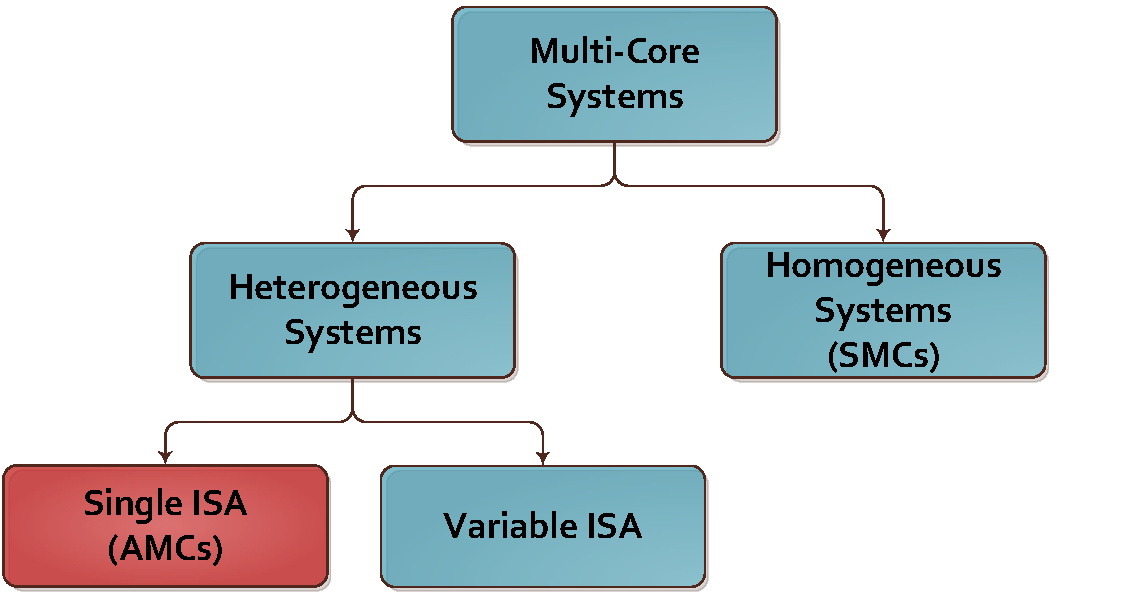
\includegraphics[width=0.7\textwidth]{figures/AMC_class.pdf}
	\caption{Classification of multi core system architectures}
	\label{fig:heterogeneous_classification}
\end{figure}
Multi-core systems can be either homogeneous or heterogeneous.
A homogeneous multi-core consists of multiple identical processing cores that have the same micro-architecture and instruction set architecture.
A heterogeneous multi-core can fall into two categories. 
The first category consists of multi-cores with different micro-architectures and ISA; systems with GPUs or other compute accelerators fall in this category.
The second category consists of of multi-cores that have different micro-architecture but a single ISA; AMC systems fall in this category.

%it can either consist of multiple cores that have different micro-architecture but a single ISA, or it can consist of multiple cores with different micro-architectures and ISA.
%Examples in the latter category include systems with GPUs or other kinds of accelerators that need to explicitly provide the code that executes on them. 

AMCs have been used in different areas of parallel computing. 
In recent years they made their appearance in the mobile market and are nowadays the most commonly used architecture for mobile processors.
The most widely used AMC architecture for mobile processors is the Arm big.LITTLE architecture~\cite{Greenhalgh2011} which combines low-power simple in-order cores (\emph{little}) with fast out-of-order cores (\emph{big}) to achieve high performance while keeping power dissipation low.
Mobile processors are also utilized in HPC platforms aiming to energy savings~\cite{ARMV8}.
%Asymmetric mobile SoCs combine low-power simple cores (\emph{little}) with fast out-of-order cores (\emph{big}) to achieve high performance while keeping power dissipation low.
Another area where AMCs have been successful is the supercomputing market.
The Sunway TaihuLight supercomputer topped the Top500\footnote{We refer to the list published inn November 2017} list in 2016 using AMCs. 
In this setup, big cores, that offer support for speculation to exploit Instruction-Level Parallelism (ILP), run the master tasks such as the OS and runtime system.
Little cores are equipped with wide Single Instruction Multiple Data (SIMD) units and lean pipeline structures for energy efficient execution of compute-intensive code. 

\kc{Challenges Using AMCs:}
AMCs are generally easy to program as the programmer does not need to express the functionality of an application for many different ISAs. 
However, there are still challenges that need to be addressed that are mainly related to the performance of the AMC.
%%Add more challenges
Like in other heterogeneous systems, load balancing and scheduling are fundamental challenges that must be addressed to effectively exploit all the resources in AMC platforms~\cite{Suleman:APLOS2009,Fedorova2009,Greenhalgh2011,Joao:ASPLOS2012,Joao:ISCA2013,ARM4HPC_SC13}. 
To preserve load balance, the system has to make sure that the cores of the system remain busy and are fairly loaded depending on their type.
For example running a barrier-based multi-threaded application where each thread runs on one core on an AMC might result in performance degradation as there is a high risk of starvation of the fast cores~\cite{AMC_survey}. %ending up in starvation. 
%the fast cores of the system will remain idle after they finish their computations waiting for the slow cores to finish execution.
%This is trivial for multi-threaded applications that run on homogeneous multi-cores but it is not as trivial on an AMC where an equal thread distribution would lead to potential starvation of the fast cores as they 

Additionally, choosing which task to execute in each type of core of an AMC is not as straightforward. 
Due to the different benefits offered by each core type, such decisions require runtime information, like task dependencies or whether a task is memory or computationally bound.
An interesting approach against the above challenges is to take advantage of the heterogeneity of an AMC by providing novel asymmetry-aware schedulers. 
%The above challenges require new asymmetry-aware scheduling approaches in order to take advantage of the heterogeneity.
The state-of-the-art asymmetry-aware scheduling approaches perform thread scheduling within the Linux kernel. 
The most commonly used example in this category is the Global Task Scheduler (GTS)~\cite{samsung} that is implemented on top of the Linux Completely Fair Scheduler (CFS) and is aware of the asymmetry of the system.
However, such approaches lack flexibility due to the high thread-migration overheads~\cite{AMC_survey}.
%Mobile applications rely on multi-programmed workloads to balance the load in the system, while supercomputer applications rely on hand-tuned code to extract maximum performance. 
%However, these approaches are not always suitable for general-purpose parallel applications.


\kc{Solutions -- mention to Task-based models and process scheduling}
The above challenges can be tackled by using task-based parallel programming models.
These parallel programming models have been widely used during the last decade in the development of parallel applications.
They form an appealing solution as they significantly ease the parallel programming by providing a higher level of abstraction to the programmer through a directive-based or language-based interface.
With these models challenges such as load balancing, scheduling, or thread migration costs are partially solved by using them out-of-the box.
They allow the programmer to split the application in multiple work units called \textit{tasks} (a function can be a task) that can potentially execute simultaneously\footnote{They can execute simultaneously given there are no task dependencies.}.
%[float, captionpos=b, caption={Pseudo-code of the task$_$finish runtime activity.},label=task_finish, emph={[2]mat}, emphstyle={[2]}, aboveskip={0\baselineskip}, frame=tb, belowskip={0\baselineskip}]
%[float, captionpos=b, caption={Example code using the OmpSs task-based programming model.}, label=task-based-example, aboveskip={0\baselineskip}, frame=tb, belowskip={0\baselineskip}]
\begin{lstlisting}[float, captionpos=b, caption={Example code using the OmpSs task-based programming model.},
label=task_finish, emph={[2]mat}, emphstyle={[2]}, 
aboveskip={0\baselineskip}, 
frame=tb]
#pragma omp task in(a) out(b)
void task1(int *a, int *b) {
  *b = *a/2 + 3 * (*a);
  return;
}
#pragma omp task in(c) inout(d)
void task2(int *c, int *d) {
  *d = 3 * (*c) + (*d) / 2;
  return;
}
int main() { 
  int x = 10, y = 5;
  for(int i = 0; i <3; i++) {
    task1(&x, &y);
    task2(&y, &x);
  }
  return 0;
}
\end{lstlisting}
As an example, Listing~\ref{task-based-example} shows a simple usage of a directive-based task-based programming model (the OmpSs programming model~\cite{OmpSs}).
In this code, the \textit{pragma omp task} directives define the functions that act as tasks, namely \texttt{task1} and \texttt{task2}.
The input and output dependencies between these tasks are derived at execution time from the \textit{in}, \textit{out} and \textit{inout} directionality clauses.
When these task functions are being called by the main function, the runtime system creates tasks that can run in parallel if there are no task dependencies between them.
The runtime system of the task-based programming model is responsible of maintaining software threads and distribute the tasks to the appropriate thread for execution.
Typically the number of software threads that the runtime system maintains is equal to the number of available cores in the system and one thread is bound to each core.
We further explain how the task-based runtime system functions in Section~\ref{sec.background.taskbased}.


\section{Thesis Motivation}
\begin{figure}[t]%
	\centering
	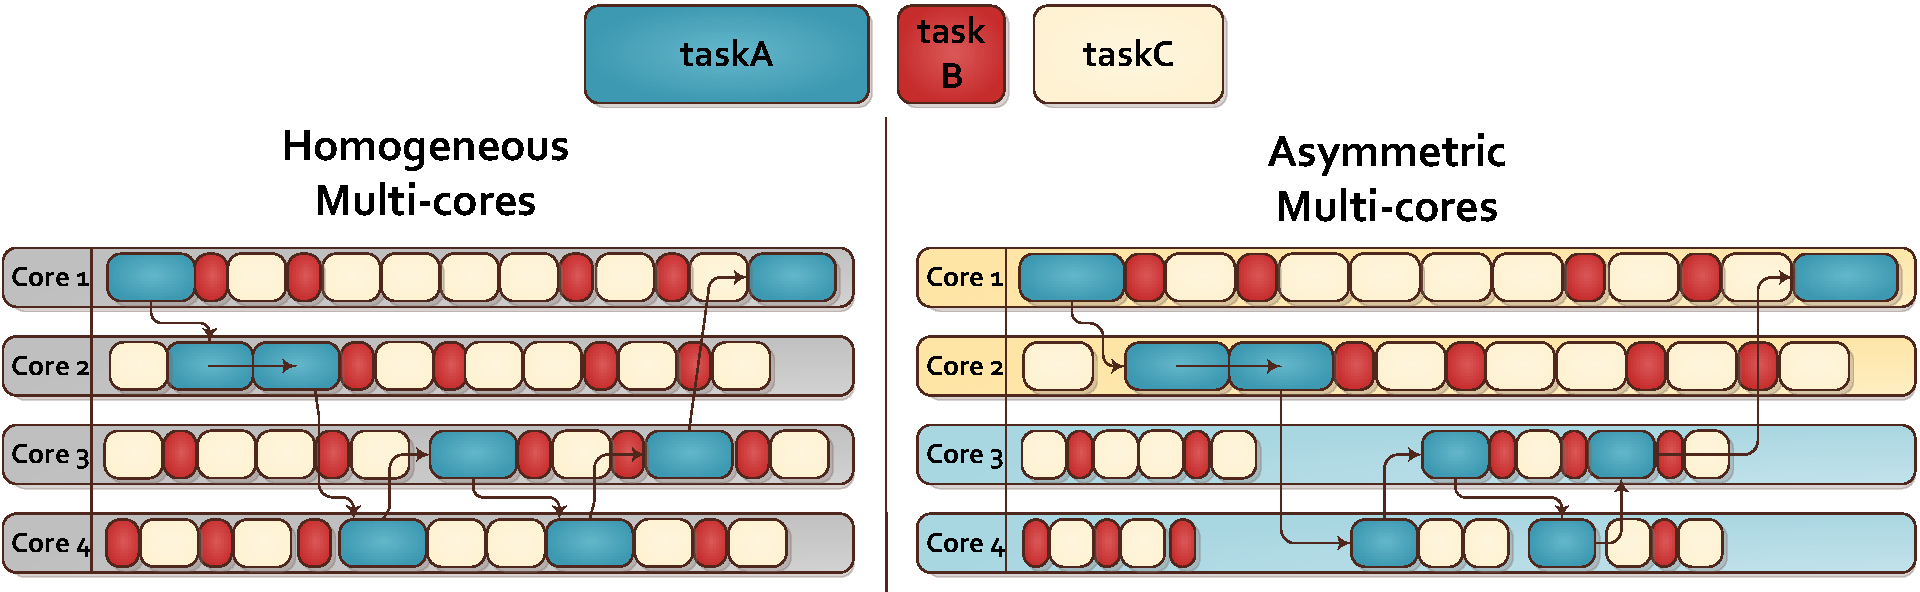
\includegraphics[width=\textwidth]{figures/thesis_motivation.pdf}
	\caption{Increased idle time when moving from homogeneous multi-core to asymmetric multi-core. The directions of the arrows indicate the data dependencies.}
	\label{fig:thesis_motivation}
\end{figure}

As was illustrated by the example of Listing~\ref{task-based-example} task-based programming models offer a very convenient abstraction layer to the programmer for parallelizing applications.
However, these parallel programming languages exhibit some challenges when moving to asymmetric systems as their runtime system is platform agnostic.
The current scheduling implementation in task-based programming models assumes that all tasks can be evenly distributed among the cores of the system and treats all tasks and cores as equal.
In some cases, a bad scheduling decision on an asymmetric system can lead to significant performance degradation. 

Figure~\ref{fig:thesis_motivation} shows the execution representation of a simple example using a task-based programming model.
This example consists of three types of tasks that have different execution times.
In this example the tasks of type taskA have dependencies between them as the arrows indicate which means that the taskA tasks cannot execute simultaneously.
The leftmost representation shows how a task-based programming model would execute this set of tasks on a homogeneous multi-core (where all cores are the same) while the representation on the right shows how the same example would execute on an asymmetric multi-core where the cores number three and four are faster than the cores number one and two.
As we can see the idle time of the cores three and four is increased when using this scheduling but this is something that can be addressed if we provide a better scheduling policy in our task-based runtime system.
Figure~\ref{fig:thesis_motivation2} shows one solution to improve this scheduling while respecting the inter-task dependencies.
\begin{figure}[t]%
	\centering
	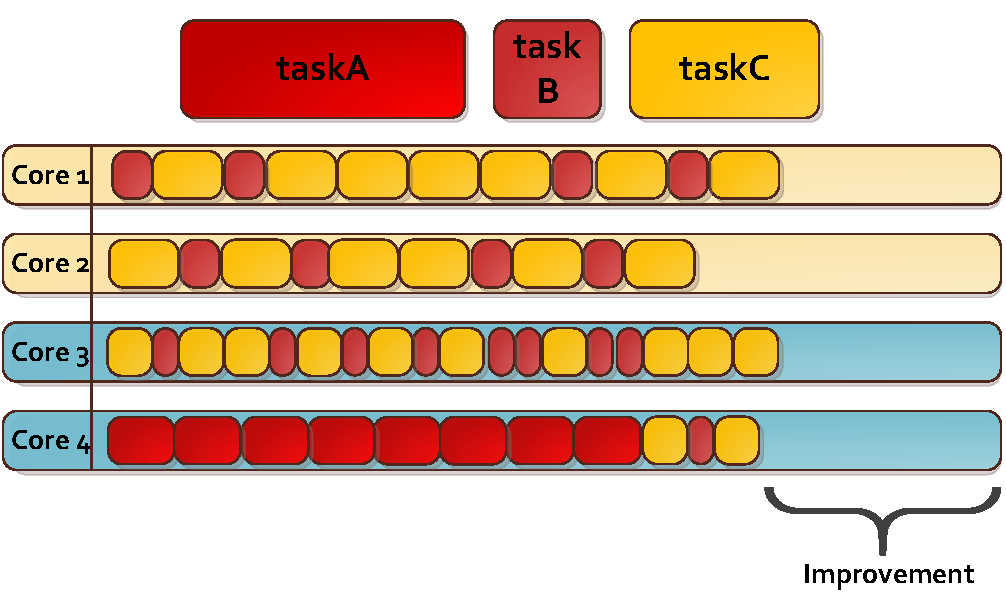
\includegraphics[width=0.65\textwidth]{figures/thesis_motivation2.pdf}
	\caption{Changing the scheduling leads to improvement for AMC systems. The directions of the arrows indicate the data dependencies.}
	\label{fig:thesis_motivation2}
\end{figure}
%A simple example is when the scheduler decides to execute a task whose output is important for the execution of a set of other tasks to one of the slow cores of the system.
%This would lead to keeping the threads idle waiting for the little core to finish the execution of this important task.

Another challenge introduced by the task-based programming models is the significant task generation overhead.
The high task generation overheads occur on both homogeneous and asymmetric multi-core systems.
Spending a lot of time on task generation can result in decreased performance as the scheduler is unable to detect the tasks and send them to the appropriate core.
The leftmost representation of Figure~\ref{fig:taskgenx_motivation} shows how the task generation affects the scheduling and increases the idle time.
The black rectangles indicate the time spent to create one task and the number inside these boxes show the task that was just created.
Looking at the yellow rectangles we can see that the execution of each task is delayed due to the delay in task generation.
The rightmost part of Figure~\ref{fig:taskgenx_motivation} shows how by reducing the task generation time scheduling of the tasks is improved and the CPU idle time is significantly reduced.
This leads to inefficient schedules with increased idle time.
Accelerating the task generation overheads increases performance of task-based programming models.

\section{Thesis Contributions}


The performance of task-based programming models can be boosted by providing sophisticated scheduling policies that take into account the platform's asymmetry.

The contributions made in this thesis rely on the efficient utilization of asymmetric multi-core systems.
Figure~\ref{fig:research_areas} shows the research areas around performance of AMC systems.
The areas shown in yellow color indicate the fields of our study.
\begin{figure}[t]%
	\centering
	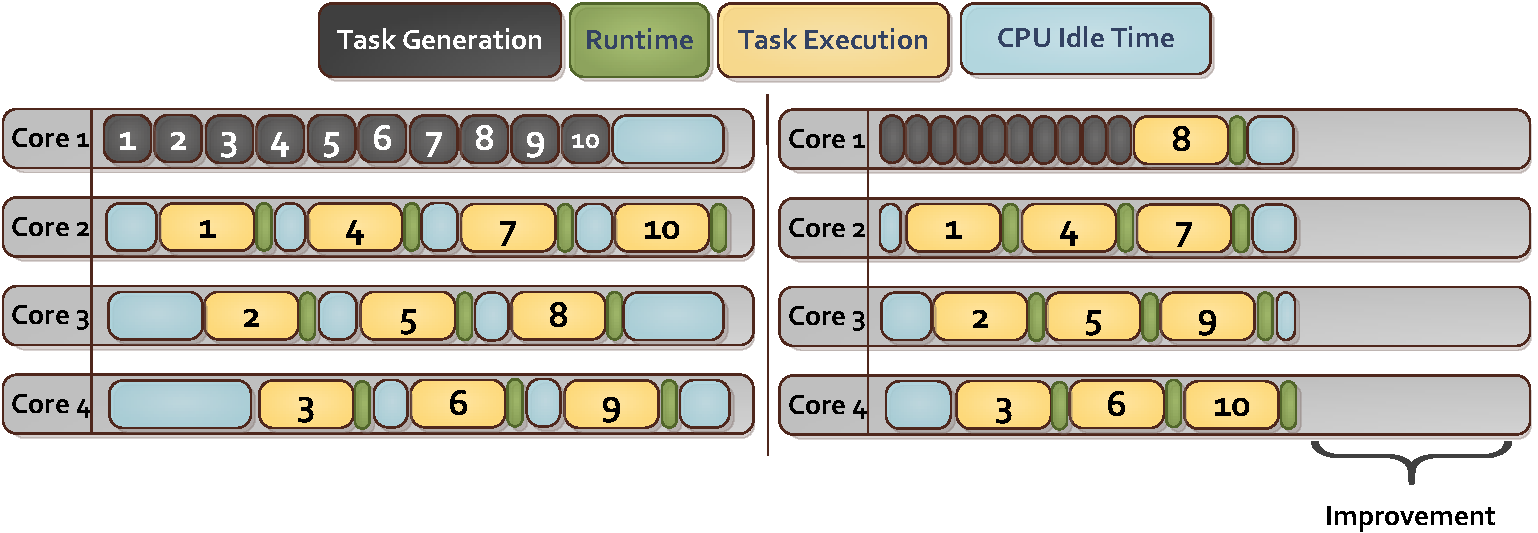
\includegraphics[width=\textwidth]{figures/taskgenx_motivation.pdf}
	\caption{Task generation overheads leads to increased idle time. Numbers inside the boxes show the task ID that is either being created or executed}
	\label{fig:taskgenx_motivation}
\end{figure}
This thesis starts with a wide experimental evaluation of highly parallel applications on AMC systems. 
We then approach the two important challenges of using task-based programming models on AMC platforms.
These challenges include first, the scheduling problem, and second the high task generation overheads introduced while using these parallel programming tools.
%which we approach by providing asymmetry-aware scheduling policies.
%The second challenge of task-based programming models is the high task generation overheads introduced while using these parallel programming tools.
%We tackle this challenge by proposing a software-hardware co-design that accelerates task generation on a specialized hardware.
Apart from scheduling within task-based programming models, this thesis includes the high-level description of a thread scheduler for asymmetric systems targeting this time mobile devices.
We tackle the above challenges and provide the following contributions:
%Below we list the contributions of this thesis:

\begin{enumerate}
	\item A thorough study of the potential of the AMC systems when running out-of-the-box HPC applications.
	We compare scheduling on different levels of the software stack and we conclude that using a task-based programming model is indeed the most efficient solution as it allows the runtime system to maintain load balance even if the system is asymmetric.
	This study serves as a verification that for HPC, scheduling through task-based programming models is indeed more efficient compared to app-based scheduling, as shown on Figure~\ref{fig:research_areas}.
	\item The design, implementation and evaluation of three novel scheduling policies that are aware of the system's asymmetry.
	These schedulers have different criteria for rating the importance of the executing tasks of an application.
	According to their distinct criteria, each scheduler identifies the \textit{critical tasks} of the application and executes them on the fast cores of the system. 
	They then leave the \textit{non-critical tasks} to be executed by the slower cores of the system.
	The research areas that were studied during at this part of the thesis are the scheduling and dependence analysis of the runtime system as shown on Figure~\ref{fig:research_areas}.
	\item The TaskGenX proposal, a hardware-software co-design scheme to reduce task generation overheads of task-based programming models.
	We implement the TaskGenX runtime system, that decouples the task generation from the other runtime activities and sends it for execution on the runtime optimized accelerator.
	Furthermore, we draw the requirements of the hardware accelerator in terms of performance with the hope to influence hardware designers for the implementation of such a component.
	The research area that is related to this contribution is the resource allocation from Figure~\ref{fig:research_areas} of the runtime systems.
	\item A high-level description of a thread scheduler for AMC systems that targets mobile devices.
	Our approach takes scheduling actions depending on the current temperature of the device and manages to increase the frames per second for three game applications while keeping the temperature stable.
	This study is briefly described due to NDA agreement as it was part of my internship in Samsung Electronics Research Institute, UK.
	This part of the thesis is within the Android framework as shown in Figure~\ref{fig:research_areas}.
\end{enumerate}


The publications that support this thesis are listed below:
\begin{enumerate}
	\item \textbf{Kallia Chronaki}, Miquel Moreto, Marc Casas, Alejandro Rico, Rosa M. Badia, Eduard Ayguade, Mateo Valero: "On the Maturity of Parallel Applications for Asymmetric Multi-Core Processors", \textit{under review, JPDC}.
	\item \cite{PACT_poster} \textbf{Kallia Chronaki}, Miquel Moreto, Marc Casas, Alejandro Rico, Rosa M. Badia, Eduard Ayguade, Mateo Valero: "POSTER: Exploiting Asymmetric Multi-Core Processors with Flexible System Software". Poster presentation in International Conference on Parallel Architecture and Compilation Techniques (PACT) 2016, Haifa, Israel.
	\item \cite{Chronaki:ICS2015} \textbf{Kallia Chronaki}, Alejandro Rico, Rosa M. Badia, Eduard Ayguade, Jesus Labarta, Mateo Valero: "Criticality-Aware Dynamic Task Scheduling for Heterogeneous Architectures".
	Paper presentation in International Conference of Supercomputing (ICS) 2015, Newport Beach, California.
	\item \cite{Chronaki:TPDS} \textbf{Kallia Chronaki}, Alejandro Rico, Marc Casas, Miquel Moreto, Rosa M. Badia, Eduard Ayguade, Jesus Labarta, Mateo Valero: "Task Scheduling Techniques for Asymmetric Multi-Core Systems". 
	Published in IEEE Transactions on Parallel and Distributed Systems (TPDS) 2017 volume 28 number 7.
	\item \cite{Chronaki:ISC} \textbf{Kallia Chronaki}, Marc Casas, Miquel Moreto, Jaume Bosch, Rosa M. Badia "TaskGenX: A Hardware-Software Proposal for Accelerating Task Parallelism".
	Paper presentation in International Supercomputing Conference (ISC) 2018, Frankfurt, Germany.
\end{enumerate}

The contributions of this paper have also been used as part of other relevant publication:
\begin{itemize}
	\item \cite{CATA} Emilio Castillo, Miquel Moreto, Marc Casas, Lluc Alvarez, Enrique Vallejo, \textbf{Kallia Chronaki}, Rosa M. Badia, Jose Luis Bosque, Ramon Beivide, Eduard Ayguade, Jesus Labarta, Mateo Valero: "CATA: Criticality Aware Task Acceleration for Multicore Processors".
	Paper presentation in IEEE International Parallel and Distributed Processing Symposium (IPDPS) 2016.
\end{itemize}
%The paper including this work, named "On the Maturity of Parallel Applications for Asymmetric Multi-Core Processors" is submitted in JPDC journal and is currently under review.
%Additionally this work was published as a poster in the conference of Parallel Architectures and Compilation Techniques in 2016 (PACT'16) with the title "POSTER: Exploiting Asymmetric Multi-Core Processors with Flexible System Software"
%
%From this contribution we had two publications; first is the "Criticality-Aware Dynamic Task Scheduling for Heterogeneous Architectures" that was presented in International Conference of Supercomputing in 2015 (ICS'15).
%The second paper including these contributions was published in the journal Transactions of Parallel and Distributed Systems in 2016 (TPDS'16) with the title "Task Scheduling Techniques for Asymmetric Multi-Core Systems".
%
%
%In this contribution 
%
%
%The paper including this contribution was published in International Supercomputing Conference on 2018 (ISC'18) with the title "TaskGenX: A Hardware-Software Proposal for Accelerating Task Parallelism".

%Apart from scheduling within task-based programming models, this thesis includes the high-level description of a thread scheduler for asymmetric systems targeting this time mobile devices.
%Our approach takes scheduling actions depending on the current temperature of the device and manages to increase the frames per second for three game applications while keeping the temperature stable.
%This study is briefly described due to NDA agreement as it was part of my internship in Samsung Electronics Research Institute, UK.
%This part of the thesis is within the Android framework as shown in Figure~\ref{fig:research_areas}.


\section{Thesis Organization}
\begin{figure}[t]%
	\centering
	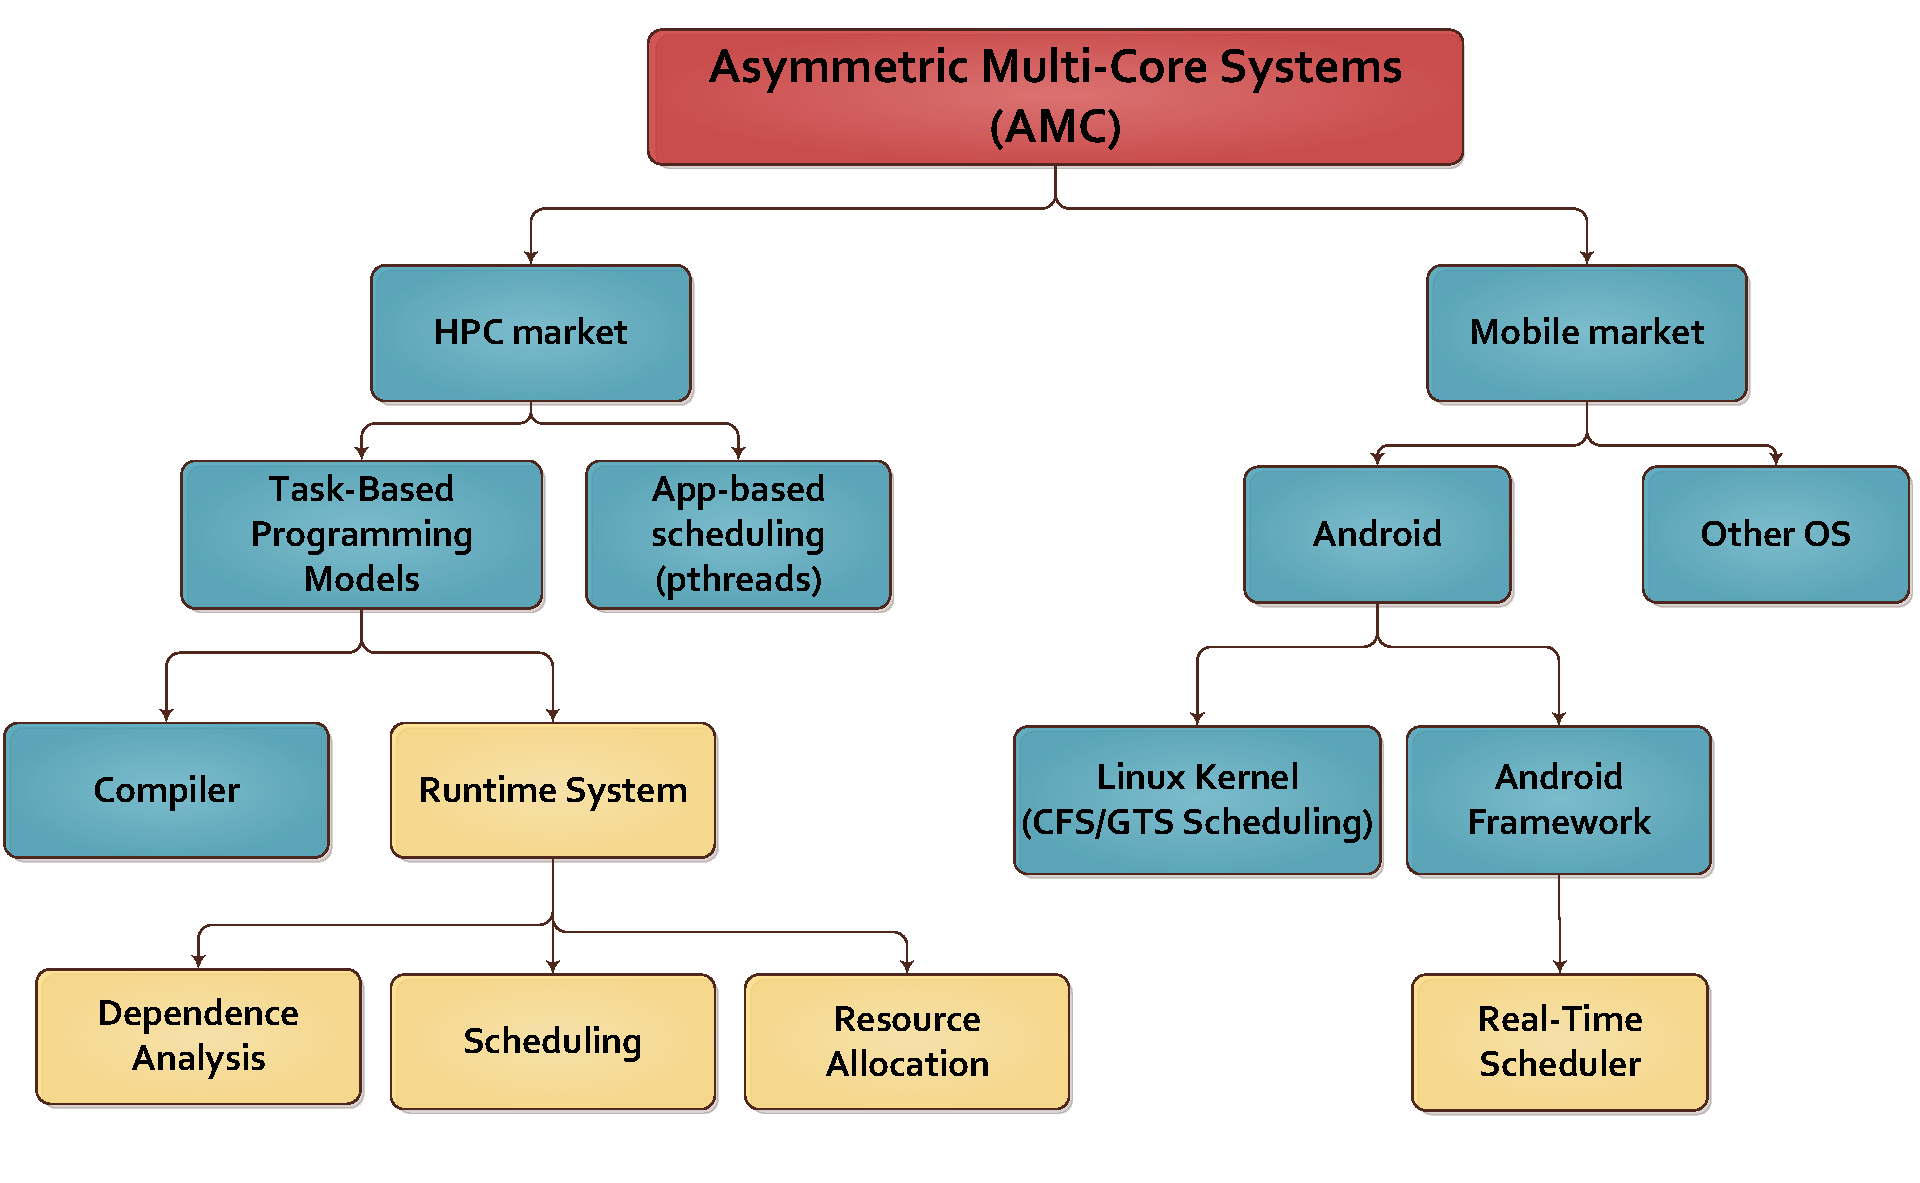
\includegraphics[width=0.7\textwidth]{figures/research_areas.pdf}
	\caption{Research areas studied in this thesis}
	\label{fig:research_areas}
\end{figure}
The rest of this document is organized as follows: 
Chapter~\ref{chapter.background} presents the background of tis thesis.
We first report the characteristics of AMC architectures, we then explain how task-based programming models are organized and how their runtime system operates, we explain a few things about the TaskSim simulator~\cite{AbstrLevels_TACO12}, that is our tool for evaluating the impact of our implementations on larger systems and finally we provide the list of applications used in our evaluation together with a short description for each one.

Chapter~\ref{chapter.study} provides our thorough and detailed study of highly parallel applications on asymmetric systems.
This study is a proof that scheduling on the runtime system is the most efficient way of utilizing an AMC system.
Chapter~\ref{chapter.scheduling} describes and evaluates our three novel scheduling approaches (CATS, CPATH and HYBRID). 
We implement these approaches within the OmpSs programming model and evaluate them using real scientific applications.
To see their impact on larger systems we use TaskSim simulator.

Chapter~\ref{chapter.taskgenx} presents our software-hardware co-design proposal, TaskGenX.
We show the implementation done and we evaluate our proposal using TaskSim simulator and real applications.
Chapter~\ref{chapter.RTS} includes the thread-based scheduling within the Android framework together with its evaluation on a mobile device using three games with intensive graphics.
Chapter~\ref{chapter.related} presents our related work and Chapter~\ref{chapter.conclusions} concludes this thesis.

%describes the evaluated AMC processor, while Section~\ref{sec:scheduling} provides information on 
%scheduling at the OS and runtime system levels. 
%Section~\ref{sec:experimental} describes the experimental framework. 
%Section~\ref{sec:evaluation} shows the performance and energy results and associated insights.% of our experiments. 
%Finally, Section~\ref{sec:related} discusses related work and Section~\ref{sec:conclusions} concludes this work. 





\iffalse
% <PACT16>

The future of parallel computing is highly restricted by energy 
efficiency~\cite{Kogge_Exascale_TR08}. Energy efficiency has become the main 
challenge for future processor designs, motivating prolific research to face the 
\emph{power wall}. Using heterogeneous processing elements is one of the 
approaches to increase energy efficiency. Different types of processors can 
be specialized for different types of computation, such as the combination of 
general-purpose cores with accelerators such as Graphics Processing Units (GPUs). 
Another approach towards heterogeneity is the use of asymmetric multi-cores 
with different types of cores with the same instruction-set architecture. Different core types 
target different performance and power optimization points for energy
efficiency~\cite{Kumar:ISCA2004,Balakrishnan:ISCA2005}. 

Asymmetric multi-cores have been successfully deployed in the mobile market, where 
low-power simple cores (\emph{little}) are combined with 
high-performance out-of-order cores (\emph{big}). Low demand applications
run on little cores for low power operation and prolong battery life. Demanding
applications, such as games, run on the big cores providing high performance
when needed.

Supercomputing is another market where asymmetric multi-cores have been successful. 
The Sunway TaihuLight supercomputer topped the Top500 list in 2016 using asymmetric multi-cores. 
In this setup, big cores, that offer support for speculation and Instruction-Level Parallelism (ILP), run the master tasks such as the OS and runtime system.
%system, as these tasks require support for speculation and Instruction-Level Parallelism (ILP) 
%exploitation of codes with complex control flow.
Little cores are equipped with wide Single Instruction Multiple Data (SIMD) units and lean pipeline structures for energy efficient execution of compute-intensive codes. 

Previous experiences have shown that load balancing and scheduling are fundamental challenges that 
must be addressed to effectively exploit all the resources in these 
platforms~\cite{Suleman:APLOS2009,Fedorova2009,Greenhalgh2011,Joao:ASPLOS2012,Joao:ISCA2013,
ARM4HPC_SC13}. 
Mobile applications rely on multi-programmed workloads to balance the load in the 
system, while supercomputer applications rely on hand-tuned code to extract maximum 
performance. However, these approaches are not always suitable for general-purpose parallel 
applications.
%In a first generation of asymmetric multi-cores, the system could switch from low power to high responding operation modes, activating or de-activating the cluster of big or little cores accordingly~\cite{ARM}. In a second generation of asymmetric multi-core processors, all the cores can run simultaneously to further improve the peak performance of these systems~\cite{samsung}.

%Many researchers are pushing towards building future parallel systems with asymmetric multi-cores~\cite{Suleman:APLOS2009,Fedorova2009, Greenhalgh2011, Joao:ASPLOS2012,Joao:ISCA2013} and even mobile chips~\cite{ARM4HPC_SC13}. However, it is unclear if current parallel applications will benefit from these asymmetric platforms. Load balancing and scheduling are two of the main challenges in utilizing such heterogeneous platforms, as the programmer has to consider them from the very beginning to obtain an efficient parallelization.

%In this paper, we evaluate for the first time the suitability of currently available mobile asymmetric multi-core platforms for general purpose computing. First, we demonstrate that out-of-the-box parallel applications do not run efficiently on asymmetric multi-cores. Fully exploiting the computational power of these processors is challenging as the asymmetry in the system can lead to load imbalance, undermining the scalability of the parallel application. Consequently, only applications that incorporate user-defined load balancing mechanisms can benefit immediately from asymmetric multi-cores.

In this paper, we evaluate several execution models on an asymmetric multi-core
using the PARSEC benchmark suite. This suite includes parallel applications from multiple domains 
such as finance, computer vision, physics, image processing and video encoding. We first quantify 
the performance loss of executing the applications \textit{as-is} on all cores 
in the system. These applications were developed on homogeneous platforms and are bound to suffer from
load imbalance on parallel regions that statically distribute the work
evenly across cores without considering their performance disparity.

Then, we evaluate several solutions at the OS and runtime level that require different
levels of user intervention to exploit asymmetric multi-cores effectively. The first
solution delegates scheduling to the OS. We evaluate the heterogeneity-aware
OS scheduler used in existing mobile platforms that assigns threads to different
core types based on CPU utilization. This requires no modification of the
application, but has limited capability for high-utilization multithreaded applications.

%on an ARM big.LITTLE asymmetric multi-core platform 

%When load-balancing techniques are not included in the original application, we evaluate alternative solutions that, without relying on the programmer, can leverage the opportunities that asymmetric systems offer. In particular, we evaluate a state of the art dynamic scheduler at the Operating System (OS) level that is aware of the characteristics of each core type. This scheduler effectively exploits the system by running high CPU utilization processes on the big cores and low CPU utilization processes on the little cores.

The second solution is to transfer the responsibility to the runtime system so it 
dynamically schedules work to different core types based on work progress and core 
availability. The advantage is that the runtime system has knowledge of the application 
structure and parallel work boundaries so it can react with certain level of predictability. 
We evaluate dynamic scheduling on top of the existing work-sharing constructs in the applications 
with an OpenMP statically-scheduled implementation available. This requires code transformations 
that are straightforward in many cases.

Finally, we evaluate the impact of using an inherently load-balanced execution model such 
that of task-based programming models. 
Recent examples~\cite{Ayguade:TPDS2009, OpenMP4.0:Manual2013, OmpSs_PPL11, Zuckerman:EXADAPT2011, Bauer.2012.SC, Vandierendonck:PACT2011, Vandierendonck:Hyperq} 
include clauses to specify inter-task dependences and remove most barriers which are the major 
source of load imbalance on asymmetric multi-cores.

%and let the runtime system to track dependences between tasks. When these dependences are satisfied, tasks are dynamically scheduled, effectively balancing the workload.

This paper quantifies the effectiveness of these solutions at different levels of the software stack
with a comprehensive evaluation of representative parallel applications on a real 
asymmetric multi-core platform: the Odroid-XU3 development board. This platform features an 
eight-core Samsung Exynos 5422 chip with ARM big.LITTLE architecture with 
four out-of-order Cortex-A15 and four in-order Cortex-A7 cores.

The rest of this document is organized as follows: Section~\ref{sec:background} describes the 
evaluated asymmetric multi-core processor, while Section~\ref{sec:scheduling} offers information on 
dynamic schedulers at the OS and runtime system levels. Section~\ref{sec:experimental} 
describes the experimental framework. Section~\ref{sec:evaluation} shows the performance 
and energy results and associated insights of our experiments. Finally, 
Section~\ref{sec:related} discusses related work and Section~\ref{sec:conclusions} concludes 
this work. 
\fi
%\begin{itemize}
% \item Out-of-the-box applications obtain the best average performance when running only on the aggressive out-of-order cores. Many of these applications are not ready to fully exploit asymmetric multi-cores as they suffer from load imbalance due to the system's heterogeneity. As a result, an average 12\% performance degradation is obtained when using all the cores in the system instead of the four out-of-order cores. 
% \item For the OS scheduler it takes three additional little cores on average to reach the performance obtained with four out-of-order cores. This is observed in most evaluated applications; the addition of little cores to a homogeneous big-core system is degrading performance. Specifically, this slowdown is observed to be 22\% on average when one little core is added to a system that consists of four big cores.
%% applications have 22\% better performance on four big cores compared to their performance on a system with four big and one little cores. 
%When adding four little cores the OS scheduler reduces total execution time by 5.3\% but contrarily to this, it is shown how the runtime system scheduling constantly improves performance by up to 16\%.
%  
%% \item Dynamic scheduling techniques at OS level can turn the tables, reducing the total execution time by 5.3\% when adding four little cores to a system with four big cores. The dynamic scheduler in the runtime system can further improve the final performance by fully utilizing all the resources in the system. This approach reaches an average 13\% speedup, and leads to the most energy efficient solution, as the Energy-Delay Product (EDP) is reduced by 40\% in this configuration.
% \item Moreover, the energy delay product (EDP) results show that the optimal solution taking into account both energy and performance remains the runtime system scheduling.
%%  In systems with a given number of out-of-order cores, adding extra in-order cores can further boost the performance of the application with the appropriate software support (at the application, runtime or OS level). As a result, the energy consumption of parallel applications running on those systems can be reduced by XXX\% on a system with four in-order and four out-of-order cores.
% \item Finally, we evaluate the usefulness of little cores to off-load runtime system activities. Similarly to the assistant core in the IBM Blue Gene Q and the Fujitsu SPARC64 XIfx processors~\cite{BG-Q:HotChips2011, Fujitsu:HotChips2014}, we explore the possibilities of devoting a little or big core to the runtime system activity. In general, we observe that the noise introduced by the runtime system does not degrade the performance of the parallel application. Thus, we can make use of this assistant core to also run user tasks, increasing the final performance of the system.
%\end{itemize}


% </PACT16>

% We describe a set of configurations for our scheduler regarding the work stealing capabilities of the different core types and the flexibility to define a task as critical or non-critical. 
 
% We implement this scheduler in OmpSs and evaluate its effectiveness on different numbers of cores and shares of fast and slow cores on a real system. 
 
% We also evaluate the effectiveness of our scheduler depending on the speed ratio between fast and slow cores using simulation.  The results show that the effectiveness of our scheduler increases with larger numbers of fast cores over slow cores, and with larger differences of performance between fast and slow cores.

%Finally, we provide a set of recommendations on how to configure our scheduler to get the best results depending on the target system size and configuration.
